\documentclass{beamer}
%\setbeamercovered{transparent}
%\usepackage{beamerthemesplit}
%\usepackage{movie15}
\usepackage{color,amsmath,xmpmulti,textpos,comment,eurosym,bm,amsthm}

%%%%%%%%%%%%%%%%%%%%%%%%%%%%%%%%%%%%%%%%%%%%%
% Lecture notes preamble
%%%%%%%%%%%%%%%%%%%%%%%%%%%%%%%%%%%%%%%%%%%%%
\input{./../../slides_preamble}

%%%%%%%%%%%%%%%%%%%%%%%%%%%%%%%%%%%%%%%%%%%%%
% LML beamer preamble
%%%%%%%%%%%%%%%%%%%%%%%%%%%%%%%%%%%%%%%%%%%%%
\newenvironment{myindentpar}[1]%
{\begin{list}{}%
    {\setlength{\leftmargin}{#1}}%
  \item[]%
}
{\end{list}}

\usetheme[hideothersubsections]{Hannover}

\newcommand\BackgroundPicture[1]{
\setbeamertemplate{background}{
\parbox[c][\paperheight]{\paperwidth}{
\vfill \hfill
\includegraphics[width=1\paperwidth,height=1\paperheight]{#1}
\hfill \vfill
}}}

\definecolor{lmlblue}{RGB}{0,70,112}
\definecolor{lmlgrey}{RGB}{142,142,142}
\definecolor{grey}{RGB}{210,210,210}

\setbeamercolor{alerted text}{fg=lmlblue}
\setbeamercolor{background canvas}{bg=white}
\setbeamercolor{block body alerted}{fg=lmlblue}
\setbeamercolor{block body}{fg=lmlblue}
\setbeamercolor{block body example}{fg=lmlblue}

\setbeamercolor{block title alerted}{fg=lmlblue}
\setbeamercolor{block title}{fg=lmlblue}
\setbeamercolor{block title example}{fg=lmlblue}

\setbeamercolor{fine separation line}{fg=lmlgrey}
\setbeamercolor{frametitle}{fg=lmlblue}
\setbeamercolor{item projected}{fg=white, bg=lmlblue}
\setbeamercolor{normal text}{fg=black}

\setbeamercolor{palette sidebar primary}{fg=lmlgrey}
\setbeamercolor{palette sidebar quarternary}{fg=lmlgrey}
\setbeamercolor{palette sidebar secondary}{fg=lmlgrey}
\setbeamercolor{palette sidebar tertiary}{fg=lmlgrey}
\setbeamercolor{section in sidebar}{fg=white}
\setbeamercolor{section in sidebar shaded}{fg=grey}

\setbeamercolor{separation line}{fg=lmlgrey}

\setbeamercolor{sidebar}{bg=lmlgrey}
\setbeamercolor{sidebar}{parent=palette primary}

\setbeamercolor{structure}{bg=white, fg=lmlblue}
\setbeamercolor{subsection in sidebar}{fg=white}
\setbeamercolor{subsection in sidebar shaded}{fg=grey}

\setbeamercolor{title}{fg=lmlblue}
\setbeamercolor{titlelike}{fg=lmlgrey}

%%%%%%%%%%%%%%%%%%%%%%%%%%%%%%%%%%%%%%%%%%%%%
% Miscellaneous preamble
%%%%%%%%%%%%%%%%%%%%%%%%%%%%%%%%%%%%%%%%%%%%%
\newcommand{\vs}[1]{\vspace{.#1cm}}
\newcommand{\vf}{\vspace{.25cm}}
\newcommand{\np}{\\ \vf}
\newcommand{\ft}[1]{\frametitle{#1}}

% add frame numbers to navigation bar
% (for RSS 2015 conference)
\addtobeamertemplate{navigation symbols}{}{
    \usebeamerfont{footline}
    \usebeamercolor[fg]{footline}
    \hspace{1em}
    \scriptsize
    \insertframenumber/\inserttotalframenumber
}

\logo{
\includegraphics[width=1.cm]{./figs/lml_square.jpg}}

\title[\insertlogo\\Lecture 4: Markets]{Lecture 4: Markets}
\author{Ole Peters\\ Alexander Adamou}
\institute{
\includegraphics[width=4cm]{./figs/lml_LOGO_whiteBG.png}}
\date{SFI Winter School\\ India, 18 December 2015}

\AtBeginSection[]{
\frame{
\ft{Agenda}
\tableofcontents[currentsection]
}
}

%%%%%%%%%%%%%%%%%%%%%%%%%%%%%%%%%%%%%%%%%%%%%
% Document
%%%%%%%%%%%%%%%%%%%%%%%%%%%%%%%%%%%%%%%%%%%%%
\begin{document}

\frame{
\titlepage
}

\frame{
\ft{Agenda}
\tableofcontents
}

%%%%%%%%%%%%%%%%%%%%%%%%%%%%%%%%%%%%%%%%%%%%%
\section{Introduction}

\frame{
\ft{Introduction}
Apply our decision theory based on time-average growth rate maximisation to markets.\np
Based on two recent papers (open access):
\bi
\item O.\ Peters. \textit{Optimal leverage from non-ergodicity.} Quant.\ Fin.\ 11 (11), 1593--1602, 2011.
\item O.\ Peters and A.\ Adamou. \textit{Stochastic market efficiency.} Santa Fe Institute working paper 13-06-022, 2013.
\ei
}

\frame{
\ft{Optimal leverage}
1. Portfolio selection problem in simple market of two assets:
\bi
\item risky asset, like a stock;
\item riskless asset, like a bank deposit.
\ei\mbox{}

How should investor allocate money between these assets (the leverage problem)?\np
Classical approach $\to$ need to know investor risk preferences.\np
Our approach: maximise $\gtm$ $\to$ unambiguous optimal leverage.
}

\frame{
\ft{Stochastic market efficiency}
2. Consider stability and efficiency of markets.\np
Does existence of objective optimal leverage constrain market prices and fluctuations?\np
Answer: yes, otherwise markets unstable and easy to beat.\np
Develop an accountable scientific theory:
\bi
\item Quantify constraint on stochastic properties of market;
\item Make prediction and account for imprecision;
\item Test against real market data.
\ei
}

%%%%%%%%%%%%%%%%%%%%%%%%%%%%%%%%%%%%%%%%%%%%%
\section{Optimal leverage}

\frame{
\ft{Model market}
Consider assets whose values follow multiplicative dynamics, which we model using GBM:
\be
d\x = \x(\gmu d\t + \gsigma d\gW).
\elabel{sde_gbm}
\ee
$\gmu$ is the drift and $\gsigma$ is the volatility.
}

\frame{
\ft{Two assets}
Simple model market of two assets.\np
\only<1>{
\underline{\textbf{Riskless}, \eg bank deposit: $\mu=\mur$; $\gsigma=0$.}\np
Investment of $\xzero$ grows deterministically:
\be
d\xzero = \xzero \mur d\t.
\elabel{sde_0}
\ee
Future value of $\xzero$ is known with certainty: 
\be
\xzero(\tn+\Dt) = \xzero(\tn)\exp(\mur\Dt). \vphantom{\left(\frac{\sigmas^2}{2}\right)}
\elabel{sde_0_soln}
\ee
$\mur$ is the riskless drift.
}
\only<2>{
\underline{\textbf{Risky}, \eg stock: $\gmu=\mus$; $\gsigma=\sigmas$.}\np
Investment of $\xone$ grows noisily:
\be
d\xone = \xone ( \mus d\t + \sigmas d\gW ).
\elabel{sde_1}
\ee
Future value of $\xone$ is a random variable:
\be
\xone(\tn+\Dt) = \xone(\tn)\exp\left[\left(\mus -\frac{\sigmas^2}{2}\right)\Dt + \sigmas \gW(\Dt)\right].
\elabel{sde_1_soln}
\ee
$\mus>\mur$ is the risky drift, $\sigmas>0$ is the volatility.
}
}

\frame{
\ft{Excess return}
The risky asset has an excess drift over the riskless asset:
\be
\mue=\mus-\mur.
\elabel{def_mue}
\ee
$\mue$ is known in finance as:
\bi
\item excess return;
\item risk premium;
\item equity premium (in context of stock markets).
\ei\mbox{}

We can view $\mue$ as compensation for accepting an uncertain outcome rather than a guaranteed result.
}

\frame{
\ft{Leverage}
How to allocate investment between the two assets?\np
Simple portfolio setup:
\bi
\item Total value $\xl$;
\item $\l\xl$ invested in stock;
\item $(1-\l)\xl$ deposited in the bank.
\ei\mbox{}

$\l$ is known as leverage.
}

\frame{
\ft{Leverage range}
$\l=0$ portfolio contains only bank deposits.\np
$\l=1$ portfolio contains only stock.\np
Not constrained to $0\leq\l\leq1$.\np
Can make $\l>1$ by borrowing money from the bank (a negative deposit) to buy stock.\np
Can make $\l<0$ by borrowing stock, selling it, and putting the proceeds in the bank (known as short selling).
}

\frame{
\ft{Leveraged SDE}
Each component of the portfolio experiences same relative fluctuations as the asset in which it was made:
\be
d\xl = \underbrace{(1-\l)\xl\vphantom{\frac{d\xzero}{\xzero}}}_\text{in bank} \frac{d\xzero}{\xzero} + \underbrace{\l\xl\vphantom{\frac{d\xzero}{\xzero}}}_\text{in stock} \frac{d\xone}{\xone}.
\ee
We already know $\frac{d\xzero}{\xzero}$ and $\frac{d\xone}{\xone}$ from the two asset SDEs.\np Substitute in to get the SDE for leveraged portfolio:
\be
d\xl = \xl [ (\mur + \l\mue) d\t + \l\sigmas d\gW ].
\elabel{sde_l}
\ee
}

\frame{
\ft{Leveraged SDE}
Value of leveraged portfolio evolves according to:
\be
\xl(\tn+\Dt) = \xl(\tn)\exp\left[\left(\mur+\l\mue-\frac{\l^2\sigmas^2}{2}\right)\Dt+\l\sigmas \gW(\Dt)\right].
\elabel{sde_l_soln}
\ee
We chose our notation for the two basic assets carefully:
\bi
\item when $\l=0$, $\xl$ evolves as $\xzero$;
\item when $\l=1$, $\xl$ evolves as $\xone$.
\ei
}

\frame{
\ft{Rebalancing}
In our model $\l$ is held constant over time.\np
Model portfolio must be rebalanced to ensure ratio of stock to total investment remains fixed.\np
Imagine stock $\downarrow$ and bank deposit $\uparrow$ over a time step.\np
Result: stock $<\l\xl$; bank deposit $>(1-\l)\xl$.\np
To restore leverage to $\l$, withdraw from bank and buy stock.\np
In the SDE we imagine this happens continuously.
}

\frame{
\ft{Question}
Simple model portfolio setup allows us to ask
\begin{keypts}{Question:}
What is the optimal value of $\l$?
\end{keypts}\mbox{}\\
Similar to the gamble problem, except we are now choosing from a continuum of gambles parametrised by $\l$.\np
Apply new decision theory $\to$ maximise time-average growth rate of investment under appropriate dynamic.
}

\frame{
\ft{Classical portfolio theory}
First let's review classical treatment of problem.\np
Intuition: there is a trade-off between risk and reward.\np
In GBM model, we might link risk to $\gsigma$ and reward to $\gmu$.\np
Ideal investment has large $\gmu$ and small $\gsigma$, but we acknowledge that larger $\gmu$ tends to come with larger $\gsigma$.\np
Hence excess return of risky over riskless asset: $\mue>0$.
}

\frame{
\ft{Efficient portfolios}
Markowitz first tried to treat this problem rigorously 1952.\np
Portfolio with $(\gsigma_i, \gmu_i)$ is ``efficient'' if no rival portfolio with $(\gsigma_j, \gmu_j)$ satisfies at least one of the statements:
\bi
\item $\gmu_j>\gmu_i$ and $\gsigma_j\leq\gsigma_i$;
\item $\gsigma_j<\gsigma_i$ and $\gmu_j\geq\gmu_i$.
\ei\mbox{}

Advice: invest only in efficient portfolios.
}

\frame{
\ft{Efficient frontier}
\only<1>{
We compare portfolios with $(\l\sigmas, \mur+\l\mue)$, which lie a on straight line in the $(\gsigma,\gmu)$-plane:
\be
\gmu = \mur + \left(\frac{\mue}{\sigmas}\right)\gsigma.
\elabel{frontier}
\ee
In Markowitz's classification, all portfolios on this line are efficient wrt to each other (known as ``efficient frontier'').\np
All leverages equally investible $\to$ no answer to our question!\np
Classical approach requires additional information to distinguish between portfolios, \eg investor risk preferences.
}
\only<2>{
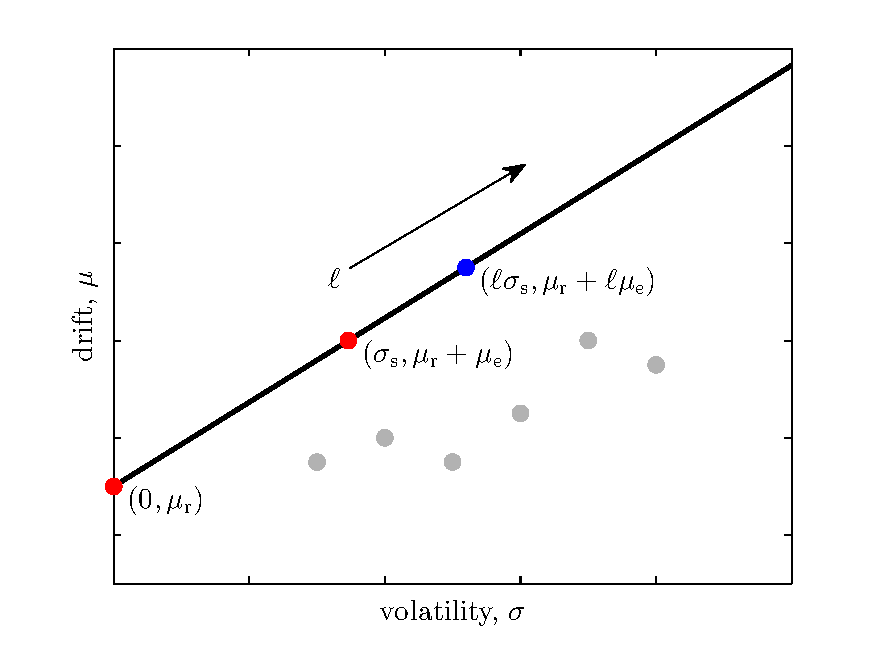
\includegraphics[width=\textwidth]{./figs/markowitz.pdf}
}
}

\frame{
\ft{Sharpe ratio}
Gradient of efficient frontier also known as the Sharpe ratio:
\be
\Sharpe = \frac{\mue}{\sigmas}.
\elabel{sharpe_l}
\ee
Shorthand for applying Markowitz's ideas: maximising $S$ is equivalent to selecting an efficient portfolio.\np
$\Sharpe$ is insensitive to $\l$ $\to$ same non-advice as Markowitz approach.
}

\frame{
\ft{Expected return}
Expected value of stock grows as
\be
\ave{\xone(\tn+\Dt)} = \ave{\xone(\tn)}\exp(\mus \Dt),
\elabel{exp_ret}
\ee
with ensemble-average growth rate or ``expected return'':
\be
\gm(\ave{\xone}) = \frac{\D\ln\ave{\xone}}{\Dt} = \mus.
\ee
Follows that expected return of leveraged portfolio is:
\be
\gm(\ave{\xl}) = \mur+\l\mue.
\elabel{exp_ret_l}
\ee
Portfolio theory insensitive to $\l$ is potentially dangerous.\np
If any $\l$ is ok, then investor maximising expected return will seek $\l\to\infty$, which will surely ruin him.
}

\frame{
\ft{Time-average growth rate}
We now understand the classical approach and its limitations.\np
What does our new decision theory have to say?\np
Time-average growth rate of leveraged portfolio is
\be
\gtm(\l) \equiv \lim_{\Dt\to\infty} \left\{ \gm(\xl,\Dt) \right\} = \lim_{\Dt\to\infty} \left\{ \frac{\D\ln \xl}{\Dt} \right\}.
\ee
Depends on $\l$. Inserting solution for $\xl(t_0+\Dt)$ gives
\be
\gtm(\l) = \lim_{\Dt\to\infty} \left\{ \frac{1}{\Dt} \left[ \left(\mur + \l\mue - \frac{\l^2\sigmas^2}{2}\right)\Dt + \l\sigmas \gW(\Dt) \right] \right\}.
\elabel{g_l_noisy}
\ee
\be
\textcolor{red}{\boxed{\;
\gtm(\l) = \mur + \l\mue - \frac{\l^2\sigmas^2}{2}.
\;}}
\elabel{g_l_quadratic}
\ee
}

\frame{
\ft{Optimal leverage}
$\gtm(\l)$ is a quadratic $\to$ unambiguous maximum at:
\be
\textcolor{red}{\boxed{\;
\lopt = \frac{\mue}{\sigmas^2}.
\;}}
\elabel{lopt}
\ee
$\lopt$ is optimal leverage which defines portfolio with fastest long-run growth $\to$ single point on the efficient frontier.\np
Only need to know $\mur$, $\mus$ and $\sigmas$ for the market assets.\np
No investor preferences (except that he maximises $\gtm$).
}

\frame{
\ft{Complete picture}
\only<1>{
$\gtm(\l)$ is time-average growth rate along the efficient frontier.\np
Time-average growth rate is $\gmu-\gsigma^2/2$ for arbitrary point in $(\gsigma, \gmu)$-plane $\to$ growth rate landscape.\np
Overlaying Markowitz picture on landscape gives missing information needed to distinguish portfolios.\np
Complete portfolio selection picture.
}
\only<2>{
\centering
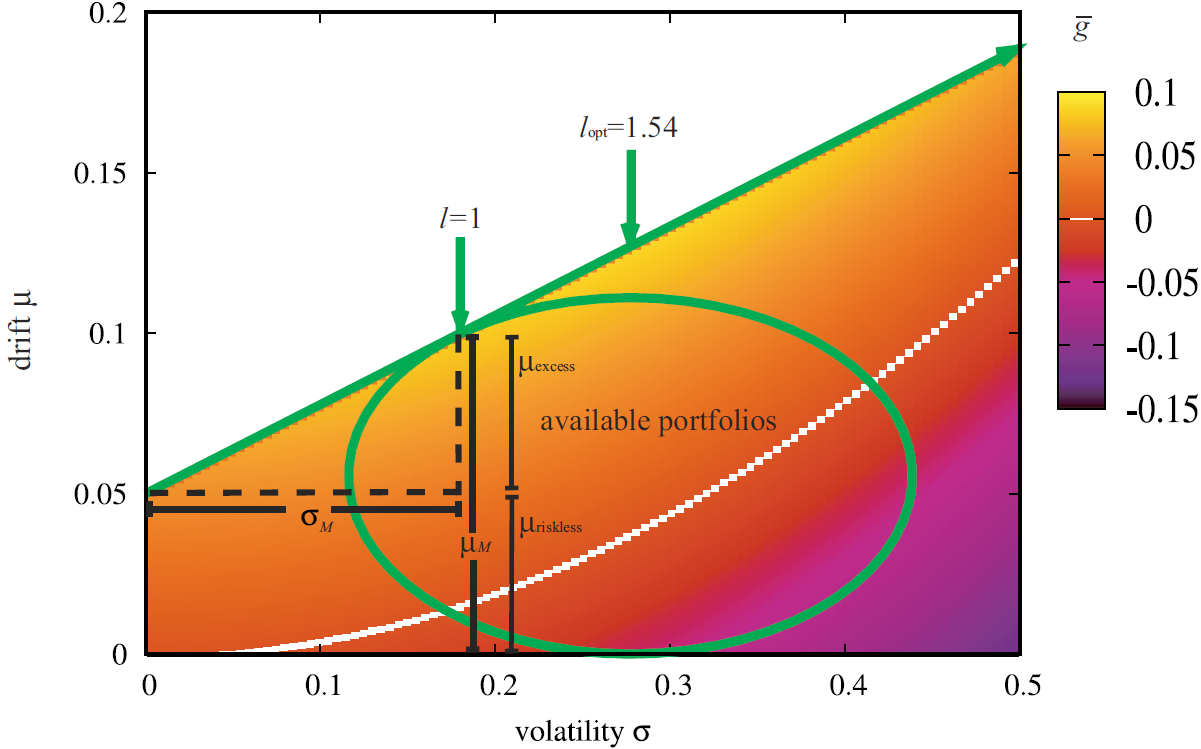
\includegraphics[width=\textwidth]{./figs/markowitz_peters.png}
}
}

\frame{
\ft{Excessive leverage}
$\gtm(\l) < 0$ for $\l<\lm$ and $\l>\lp$, where
\be 
\lpm = \lopt \pm \sqrt{\lopt^2 + \frac{2\mur}{\sigmas^2}}
\ee
are the roots of $\gtm(\l)=0$.\np
Investor maximising $|\l|$ in either direction will cause his wealth to decay rapidly:
\be
\gtm(\l)\to-\infty \quad\text{as}\quad |\l|\to\infty.
\ee
}

%%%%%%%%%%%%%%%%%%%%%%%%%%%%%%%%%%%%%%%%%%%%%
\section{Stochastic market efficiency}

\frame{
\ft{Fundamental measure}
$\Sharpe=\mue/\sigmas$ is a dimensionful quantity: $(\text{time unit})^{-1/2}$.\np
Value depends on time unit $\to$ arbitrary, \eg $\Sharpe=5\text{ y}^{-1/2}$ $\approx 0.26\text{ d}^{-1/2}$. Same portfolio, different numbers.\np
Tells us nothing fundamental about system under study.\np
$\lopt=\mue/\sigmas^2$ is a dimensionless quantity.\np
Value does not depend units and can carry fundamental information about system.\np
View $\lopt$ as fundamental measure of portfolio quality.
}

\frame{
\ft{Question}
However, significance of $\lopt$ runs deeper than this.\np
Optimal allocation of investment between risky and riskless assets in model market $\to$ tells us about market conditions.\np
High $\lopt$ indicates environment in risk-taking is incentivised. Low/negative $\lopt$ indicates the converse.
\begin{keypts}{Question:}
Are there any special values of $\lopt$ which describe different market regimes, or to which markets are attracted?
\end{keypts}
}

\frame{
\ft{Relaxing the model}
Assets in model market have static $\mur$, $\mus$, $\sigmas$ $\to$ static $\lopt$.\np
Hard to explore question if $\lopt$ can't vary $\to$ need to relax model to make progress.\np
Real market assets don't follow GBM with static parameters.\np
In particular, real market conditions -- represented in model by $\mur$, $\mus$, $\sigmas$ -- change slowly (wrt to fluctuations).\np
Relax model constraint of static parameters and allow them to vary $\to$ allow $\lopt$ to change over time.
}

\frame{
\ft{Classical efficiency}
In general, an efficient system is one which is well optimised and can't be improved by simple actions.\np
Classical ``efficient market hypothesis'' treats markets as information processors (\eg Hayek 1945, Fama 1965).\np
Claim: price of asset in efficient market accurately reflects all publicly available information.\np
Corollary: no market participant, without access to privileged information, can consistently beat the market simply by choosing prices at which he buys and sells.
}

\frame{
\ft{Thought experiment}
Consider a different efficiency involving leverage rather than price/information. Start with a thought experiment\ldots\np
Imagine $\lopt>1$ in our model market:\np
$\to$ Simple strategy of borrowing money to buy extra stock will achieve faster long-run growth than full investment in stock.\np
$\to$ Trivial matter for us to beat the market.\np
Similarly, imagine $\lopt<1$: again easy to beat market by leaving some money in the bank (and, if $\lopt<0$, short selling).
}

\frame{
\ft{Stochastic efficiency}
Hard to call a market efficient if it's so easy to beat.\np
Suggests different notion of efficiency $\to$ stochastic efficiency.\np
Claim: impossible for participant to beat a stochastically efficient market simply by applying leverage.
\begin{keypts}{Hypothesis: stochastic market efficiency (strong form)}
Real markets self-organise such that
\be
\boxed{\; \lopt = 1 \;}
\elabel{sme_strong}
\ee
is an attractive point for their stochastic properties (represented by $\mur$, $\mus$, $\sigmas$ in the relaxed model).
\end{keypts}
}

\frame{
\ft{Stability}
Another approach: consider market stability and its dependence on $\lopt$. Run another thought experiment\ldots\np
\underline{Imagine $\lopt>1$:}\np
Objectively optimal $\to$ \textit{everyone} in market should want to borrow money to buy stock.\np But, if so, who will lend money and who will sell stock?\np
\underline{Imagine $\lopt<0$:}\np
\textit{Everyone} should want to borrow stock and sell it for cash.\np
But who will lend stock and who will relinquish cash to buy it?
}

\frame{
\ft{Stable range for $\lopt$}
Neither situation globally stable: $0\leq\lopt\leq1$ is stable range.\np
Hard to imagine deviations persisting for long before trading changes market parameters to return $\lopt$ to stable value.\np
\begin{keypts}{Hypothesis: stochastic market efficiency (weak form)}
Real markets self-organise such that
\be
\boxed{\; 0\leq\lopt\leq1 \;}
\elabel{sme_weak}
\ee
is an attractive range for their stochastic properties.
\end{keypts}
}

\frame{
\ft{Self-organisation}
Self-organisation of parameters occurs \textit{via} trading activity.\np
Feedback loops dynamically adjust prices and fluctuations to pull $\lopt$ back to stability when it strays.\np
Detailed mechanisms can be found in Peters \& Adamou 2013.\np
Strong hypothesis favoured over weak as expect $\l=0$ a weaker attractor than $\l=1$ (to avoid economic paralysis).
\begin{keypts}{Hypothesis: stochastic market efficiency (refined)}
On sufficiently long time scales, $\lopt=1$ is a strong attractor for the stochastic properties of real markets. Deviations from this attractor over shorter time scales are likely to be confined to the range $0\leq\lopt\leq1$.
\end{keypts}
}

\frame{
\ft{Tests of the hypothesis}
Test by simulating leveraged investments in a real stock market.\np
Treat U.S.\ S\&P500 index as real-world equivalent of risky asset.\np
Treat bank deposits at historical interest rates as real-world equivalent of riskless asset.\np
Historical period: August 1955 to May 2013.
}

\frame{
\ft{Data sets}
\bc

\includegraphics[width=0.5\textwidth]{./figs/fred.png}
\ec
Use FRED time series:
\bi
\item \texttt{SP500} -- daily closing prices of S\&P500;
\item \texttt{DFF} -- effective federal funds rate;
\item \texttt{DPRIME} -- bank prime loan rate.
\ei\mbox{}

S\&P500 $\to$ well diversified portfolio of large and successful companies $\to$ generous estimate of $\lopt$.
}

\frame{
\ft{Simulation}
Simulate investment of constant leverage over time window:
\bi
\item Assume net value (equity) of $\$1$ at start of window: $\$\l$ in S\&P500; $\$(1-\l)$ in bank;
\item Update values of each component daily according to historical returns and rebalance portfolio;
\item If equity falls below zero, investment is bankrupt and simulation stops;
\item Proceed to last day of the window and record final equity.
\ei\mbox{}

Repeat simulation for different $\l$ to find simulated optimal leverage, $\lopts$, which maximises final equity.
}

\frame{
\ft{Full time series}
\only<1>{
\centering
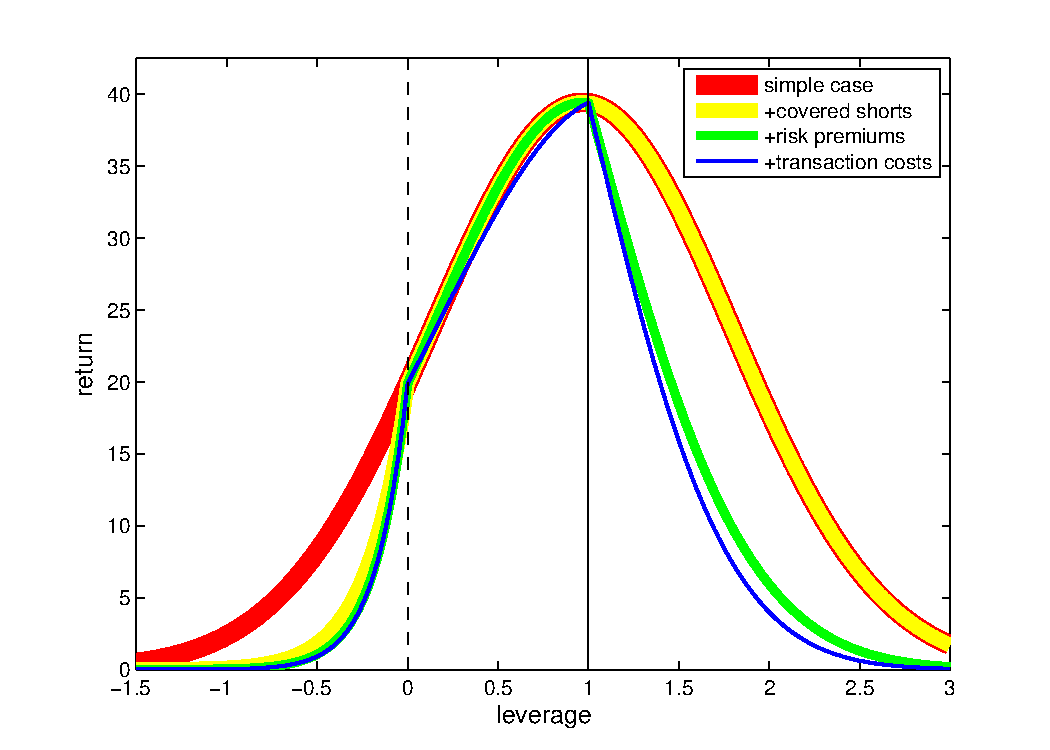
\includegraphics[width=\textwidth]{./figs/sme_fig1.pdf}
}
\only<2>{
Simulated return-leverage curves correspond to different sets of assumptions about interest rates and transaction costs.\np
Labelled 1--4 in increasing complexity and resemblance to real market practices (call 1 ``simple'' and 4 ``complex'').\np
$\lopt\approx0.97$ for simulations 1--3.\np
$\lopt=1.00$ for simulation 4!\np
Results consistent with stochastic efficiency -- discuss statistical significance shortly.
}
}

\frame{
\ft{Parabolic fit}
\only<1>{
\centering
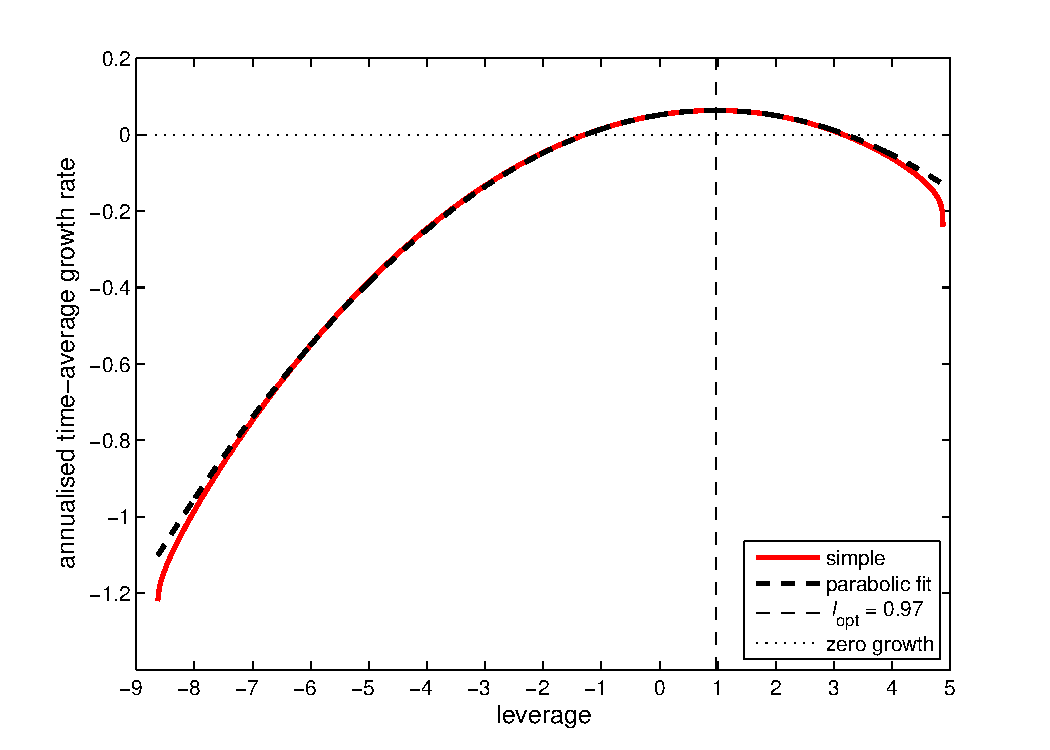
\includegraphics[width=\textwidth]{./figs/sme_fig2.pdf}
}
\only<2>{
For $\Dt=58$ years, expect simulated growth rate $\approx\gtm(\l)$.\np
Parabolic form of GBM-based model clearly visible in plot.\np 
Parameters of fitted parabola give effective values of $\mur$, $\mue$, $\sigmas$ for S\&P500 over time series.\np
Least-squares fit:
\bi
\item $\mur=5.2\%$ \textit{pa};
\item $\mue=2.4\%$ \textit{pa};
\item $\sigmas=16\%$ \textit{p$\sqrt{\mathit{a}}$}.
\ei
}
\only<3>{
Deviation from parabolic form for high and low leverages due to extreme fluctuations.\np
$\to$ Large losses and bankruptcy for high leverage portfolios.\np
Common criticism is that: real return distributions have fatter tails than in models.\np
Not relevant here: large deviations strengthen stochastic efficiency hypothesis because they penalise high leverage.
}
}

\frame{
\ft{Equity premium puzzle}
Results relevant to unexplained phenomenon in economics: the ``equity premium puzzle''.\np
Claim: observed equity premium ($\mue$ in model) incompatible with theory as it implies investors implausibly risk averse.\np
6\% \textit{pa} established in literature \textit{vs.}\ 2.4\% \textit{pa} in our model.\np
Source of discrepancy unclear because classical estimates based on complicated behavioural models.\np
No puzzle in our model: $\mue$ consistent with stochastic efficiency.
}

\frame{
\ft{Finite time scales}
Can't observe $\gtm(\l)$ as this requires infinite observation time.\np
Can only observe finite-time growth rate $\gm(\xl,\Dt)$ over simulation window $\Dt$.\np
Random variable whose distribution broadens as $\Dt\to0$.\np
Also can't observe $\lopt$ but only simulated optimal leverage $\lopts(\Dt)$ which maximises $\gm(\xl,\Dt)$.\np
$\gm(\xl,\Dt)$ worse estimator of $\gtm(\l)$ as $\Dt\to0$, so $\lopts(\Dt)$ worse estimator of $\lopt$.
}

\frame{
\ft{Significance}
\only<1>{
When is a single observation of $\lopts(\Dt)$ consistent with our hypothesis significant?\np
Depends on width of distribution of $\lopt(\Dt)$:
\bi
\item if width much larger than hypothesised stable range of $\lopt$, then can't read much into one observation;
\item if width similar to or smaller than stable range, then observation outside is strong evidence that hypothesis is flawed, so observation inside significant.
\ei
}
\only<2>{
Quantify these ideas in original model:
\be
\gm(\xl,\Dt) = \mur+\l\mue-\frac{\l^2\sigmas^2}{2}+\frac{\l\sigmas \gW(\Dt)}{\Dt}.
\elabel{g_l_finite}
\ee
\be
\Rightarrow \quad \lopts(\Dt) = \lopt + \frac{\gW(\Dt)}{\sigmas\Dt}.
\elabel{lopt_finite}
\ee
Normally distributed with mean $\lopt$ and standard deviation:
\be
\text{stdev}[\lopts(\Dt)] = \frac{1}{\sigmas\sqrt{\Dt}}.
\elabel{lopt_sd}
\ee
For $\Dt\approx58$ years and fitted $\sigmas$, get $\text{stdev}[\lopts(\Dt)]\approx0.83$.\np
So single observation is significant corroboration of hypothesis.
}
}

\frame{
\ft{Fluctuations}
Test model prediction by running simulations with different window lengths and compiling histograms of $\lopts(\Dt)$:
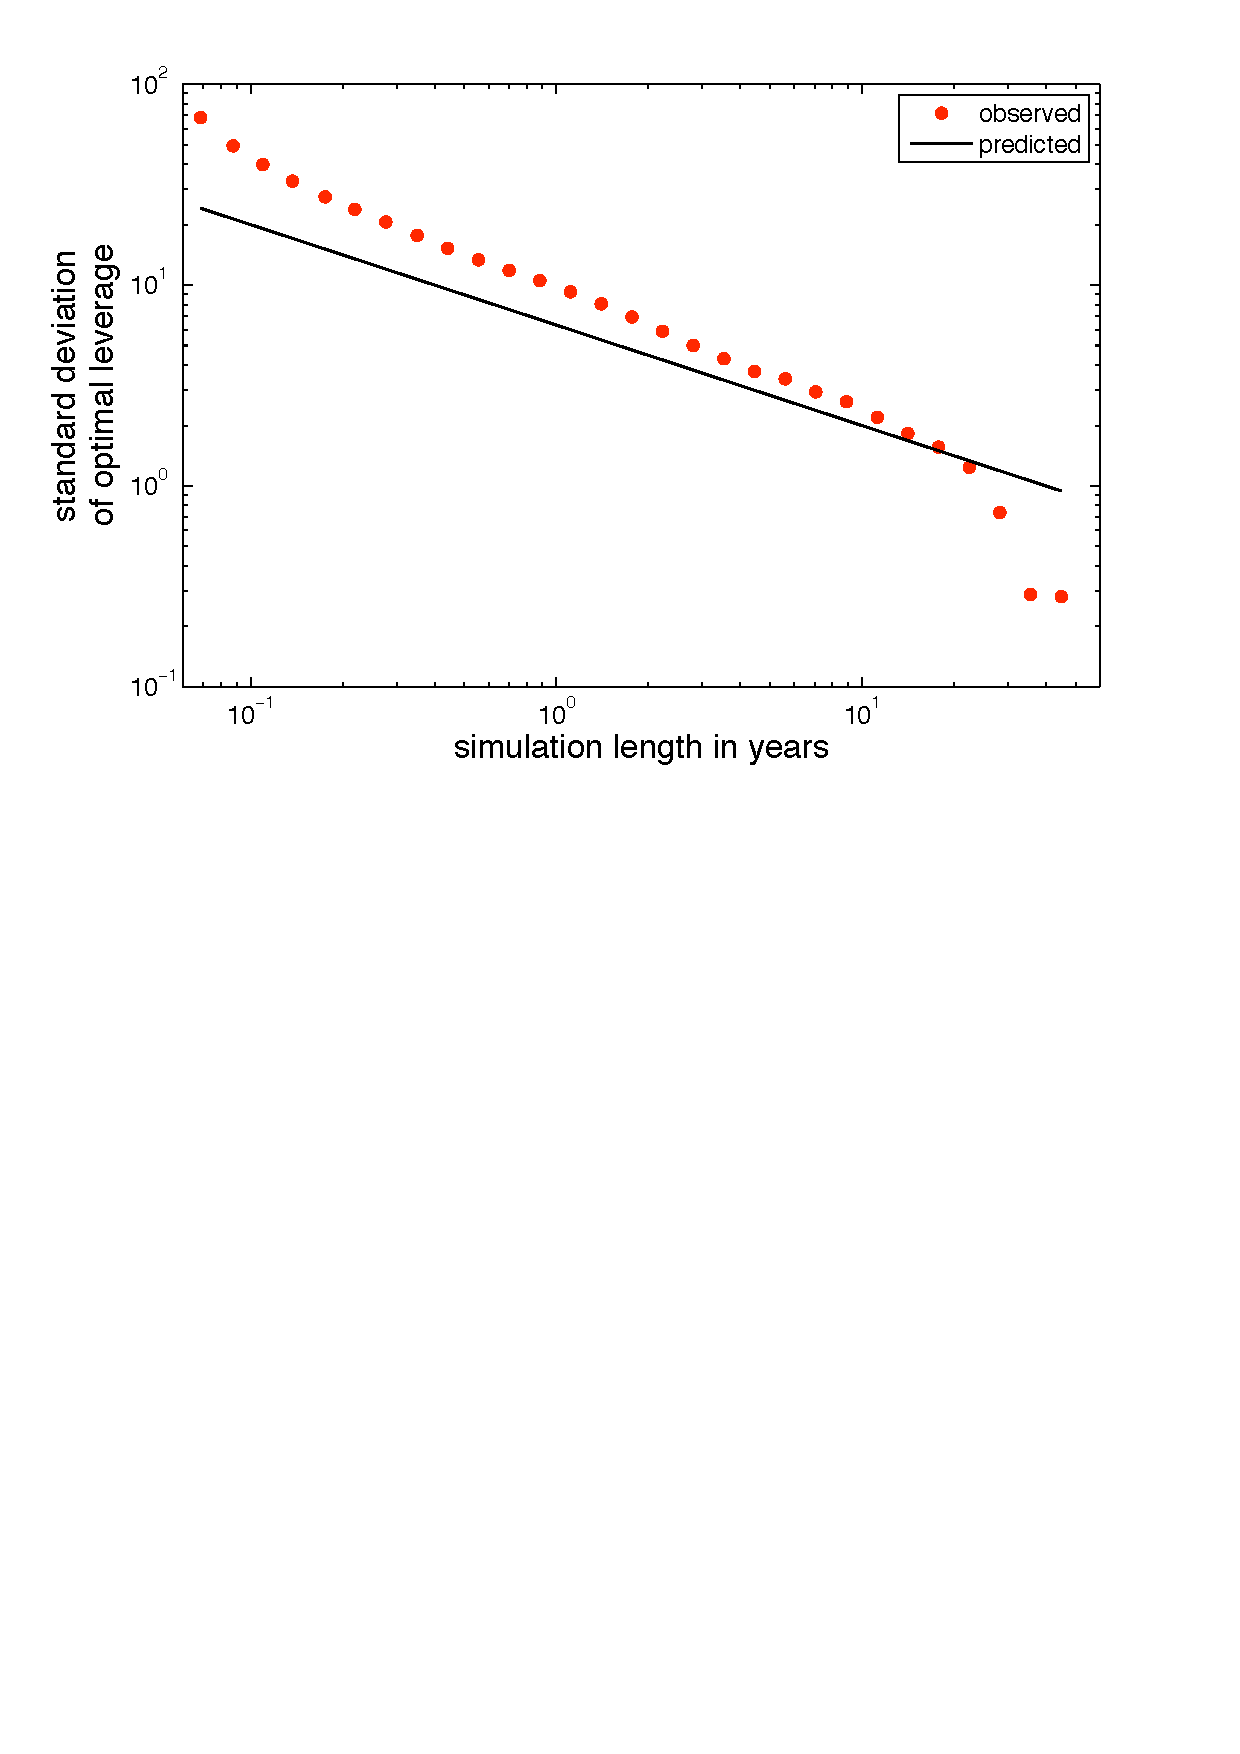
\includegraphics[width=\textwidth]{./figs/sme_fig3.pdf}
}

\frame{
\ft{Expanding window}
\only<1>{
Run simulations starting on first day of time series with increasing window lengths.\np
Reduced fluctuations in $\lopts(\Dt)$ with increasing window length consistent with model.\np
Evolution of $\lopts(\Dt)$ supports hypothesis that $\lopt$ attracted to range $0\leq\lopt\leq1$ and, over long time scales, to $\lopt=1$.
}
\only<2>{
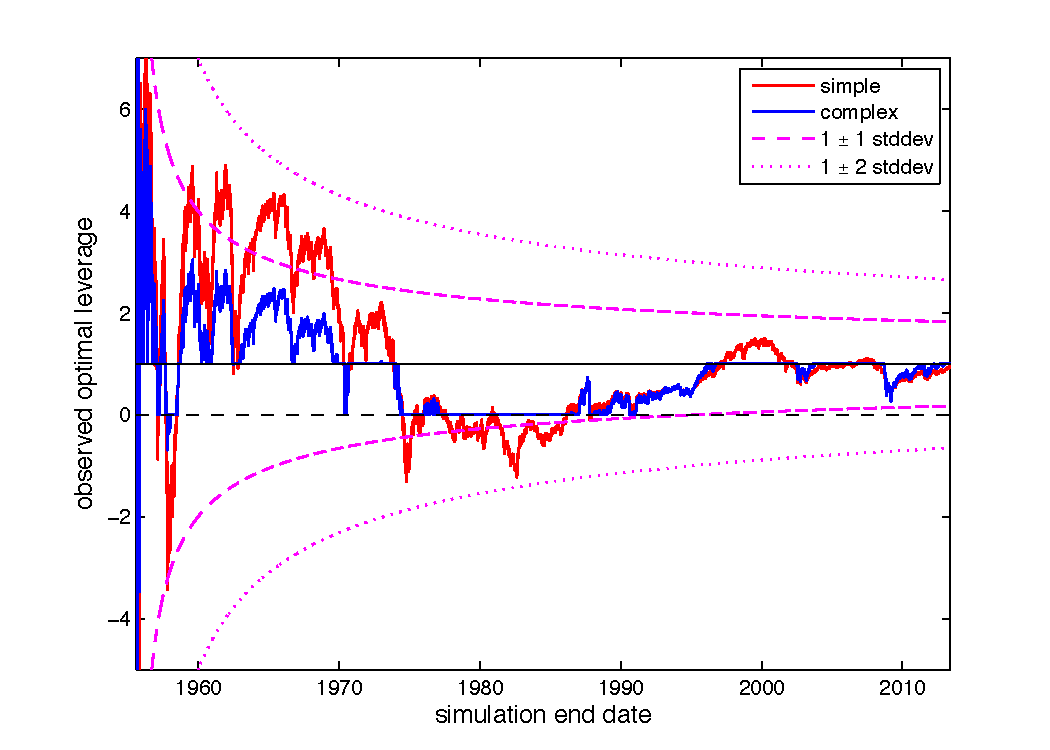
\includegraphics[width=\textwidth]{./figs/sme_fig4.pdf}
}
}

\frame{
\ft{Moving windows}
\only<1,4>{
Can also plot $\lopts(\Dt)$ for windows with fixed lengths and moving start date.\np
Run simple and complex simulations with window lengths ranging from 5 to 40 years\ldots\np
}
\only<2>{
Simple simulation:
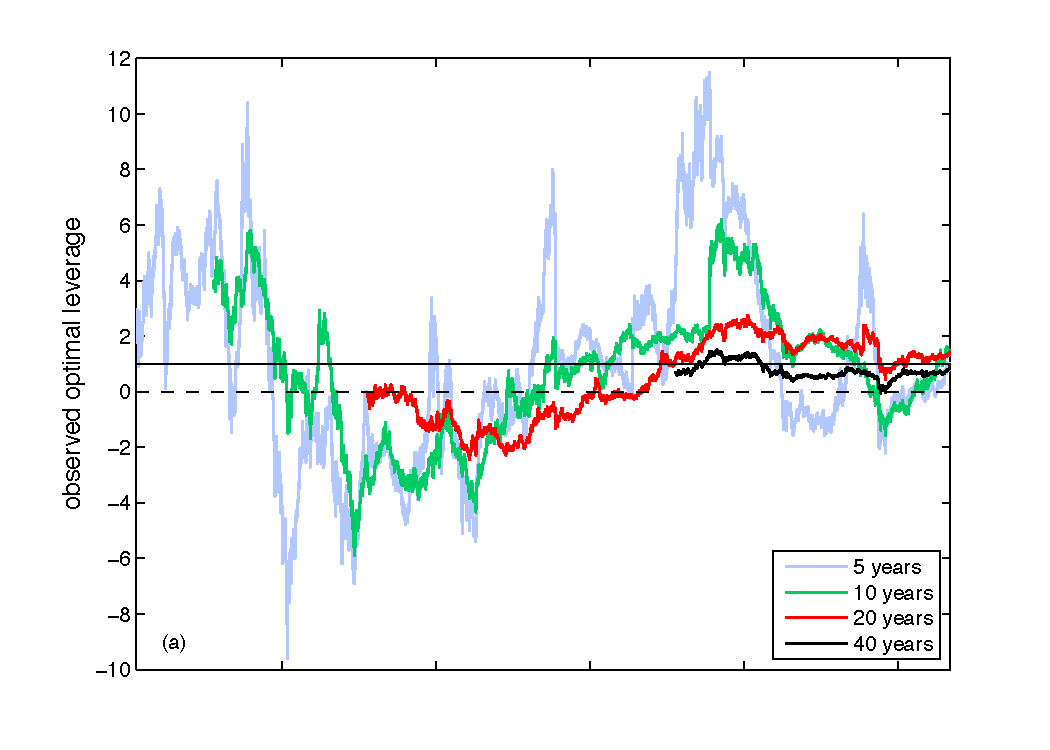
\includegraphics[width=1.\textwidth]{./figs/sme_fig5a.pdf}
}
\only<3>{
Complex simulation:
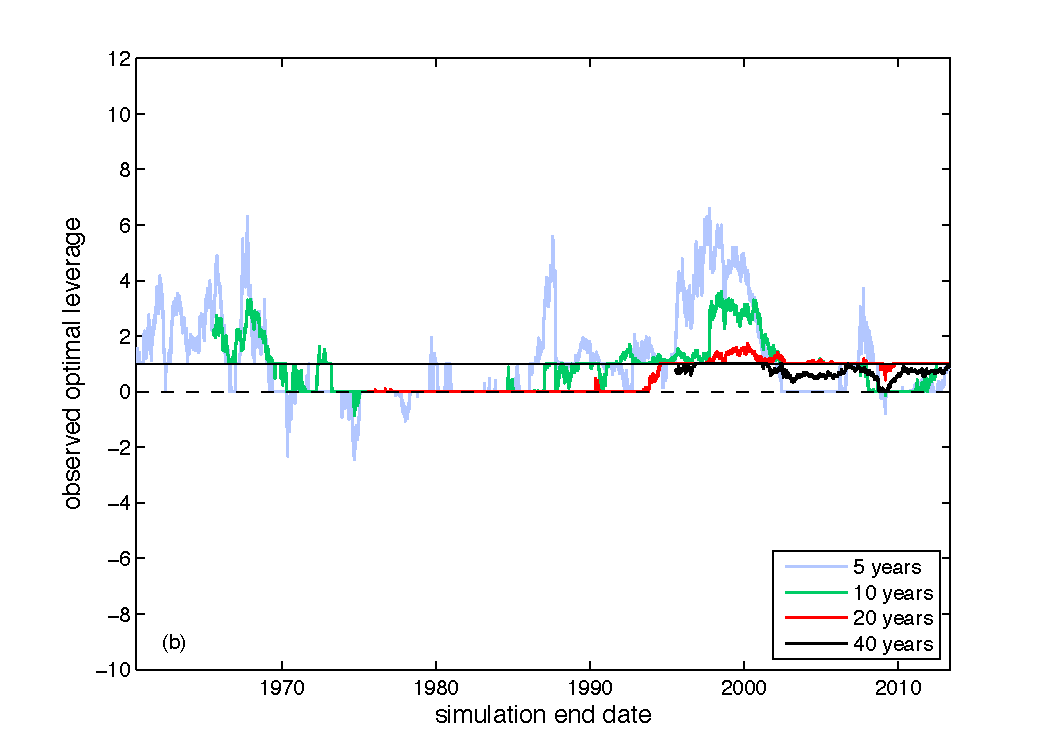
\includegraphics[width=1.\textwidth]{./figs/sme_fig5b.pdf}
}
\uncover<4>{
\underline{Observe:}
\bi
\item Strong fluctuations over short time scales;
\item Weak fluctuations over long time scales;
\item Attractive behaviour consistent with refined hypothesis.
\ei
}
}

\frame{
\ft{Discussion}
Mathematical formalism developed to conceptualise randomness in economics is very powerful.\np
Does more than just create a foundation for economic theory.\np
Framework is epistemologically sound $\to$ make testable predictions, \eg stochastic efficiency.\np
Hard to guess from coin-tossing game that we could predict stochastic properties of U.S.\ stock market over 58 years!\np
What other surprising predictions can we make in this formalism?
}

\end{document}